%! Author = Saeid Yazdani
%! Date = 8/15/2024


\section{Compensation Unit}
\label{sec:compensation-network}

The control loop can be characterized by frequency response on the output and
a compensation network is necessary for maintaining the stability, response
time, and performance of the feedback loop that regulates the output voltage or
current under various load conditions.

There are several ways to achieve the best-case compensation.
In the first approach, we don't change the amplifier's compensation during
the control loop calculations.
Instead, compensation is provided by an RC network and a set of electronic
relays, which help to optimize the control loop's behavior.
In the subsequent step, the compensation network can be adjusted on the fly,
leading to a more optimized step response.

\subsection{Static Compensation}
\label{subsec:static-compensation}

The two registers, PRECMP\_C (pre-amplifier compensation capacitor array) and
PRECMP\_R (pre-amplifier compensation resistor array), define the static
settings for compensation.
Additionally, there are PACMP\_C (power-amplifier compensation capacitor array)
and PACMP\_R (power-amplifier compensation resistor array) for extra
compensation of the power amplifier, even though the power amplifier may not
require variable compensation during runtime.
Clearing the CONFIG\_REG[14] bit enables online compensation.
In the initial approach, we maintain all compensation settings as constant
(the slowest version).
Static compensation can then be adjusted based on the results of the system
characterizations after production.

\subsection{Dynamic Compensation}
\label{subsec:dynamic-compensation}

Dynamic compensation involves modifying the compensation settings at
specific points in time and is the basis for the adaptive-predictive
compensation discussed in \autoref{subsec:time-variant-comp-network}.

For each timing event, we have a set of corresponding timing registers,
TIM\_0 to TIM\_7.
When the internal counter reaches the value set in the first timing register,
the corresponding compensation settings are applied.
This process continues sequentially through up to eight register sets.

By default, the dynamic compensation scheme is active and can be disabled by
clearing the CONFIG\_REG[14] bit (switch to static compensation mode).
The internal counter begins from zero, triggered by a signal when a new SET
value is generated (a short pulse to logic level 1, then immediately returning
to zero).

Dynamic compensation settings are designed to optimize the transition
times for output signals.
As the output signal approaches the target value, the initial rise time is
reduced, minimizing overshoot and ensuring a smooth entry into the tolerance
band.

\subsection{Compensation Control in the \acs{FPGA}}
\label{subsec:compensation-control-fpga}

The dynamic compensation system functions by selectively engaging and
disengaging arrays of resistors and capacitors.
Given that modifying the compensation network is a time-critical task,
the decision-making algorithm is implemented within the FPGA logic.
This implementation allows for timely control of the R/C arrays via
FPGA's GPIO pins, eliminating the need for \ac{MCU} and associated bus-access
overhead.

\autoref{tab:compensattion-registers-fpga} shows the dedicated registers
for controlling the compensation networks.

\begin{table}[h]
    \centering
    \resizebox{\linewidth}{!}{%
    \begin{tabular}{|>{\centering\arraybackslash}m{0.2\textwidth}|>{\centering\arraybackslash}m{0.2\textwidth}|>{\centering\arraybackslash}m{0.1\textwidth}|>{\centering\arraybackslash}m{0.05\textwidth}|>{\centering\arraybackslash}m{0.35\textwidth}|}
        \hline
        \text{Address (dec)} & \text{Address (hex)}            & \text{Bits} & \text{Type} & \text{Desciption}      \\
        \hline
        64 - 71              & \texttt{0x40} .. \texttt{0x47}  & 8           & RW          & Pre-amplifier 0 to 7   \\
        \hline
        72 - 79              & \texttt{0x48} .. \texttt{0x4F}  & 8           & RW          & Power Amplifier 0 to 7 \\
        \hline
        80 - 87              & \texttt{0x500} .. \texttt{0x57} & 8           & RW          & Timing 0 to 7          \\
        \hline
    \end{tabular}
    }
    \caption[Compensation Registers]{
        Compensation Registers in the \acs{FPGA}
    }
    \label{tab:compensattion-registers-fpga}
\end{table}


Each timing register specifies the exact moment when the values from the
compensation register are applied. When a new value is written, compensation
is initially set to its minimum.
An internal counter, starting from 0, continuously compares its value with the
timing registers 0 through 7.
When a match is found, the corresponding compensation setting is activated
by switching control relays using \acs{FPGA}'s \acs{GPIO} pins.
This procedure is depicted in \autoref{fig:compensation-apply-timing}
and \autoref{fig:compensation-arrangement}.

At system startup, the microcontroller is responsible for configuring all
settings and writing them into 24 registers.
These values are independent of the applied voltage and current ranges; they
must be fine-tuned during the characterization of \acs{HVS} after production.


\begin{figure}[t!]
    \centering
    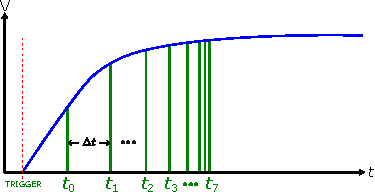
\includegraphics[width=0.6\textwidth]
    {figures/design-realization/compensation-apply-timing}
    \caption[Compensation Apply Timer]{
        The compensation network is set within 8 discrete steps.
        The timing between steps is customizable through TIM\_0 to TIM\_7 registers
        and a resolution of \SI{1}{\nano\second} is theoretically possible and is
        subject to the speed of analog switches used in the circuit.
        The reset values of timing registers are as follows:
        \SI{44.8}{\micro\second}, \SI{22.4}{\micro\second},
        \SI{11.2}{\micro\second}, \SI{5.6}{\micro\second},
        \SI{2.8}{\micro\second}, \SI{1.4}{\micro\second},
        \SI{0.7}{\micro\second}, \SI{0.4}{\micro\second}
    }
    \label{fig:compensation-apply-timing}
\end{figure}

\begin{figure}[t!]
    \centering
    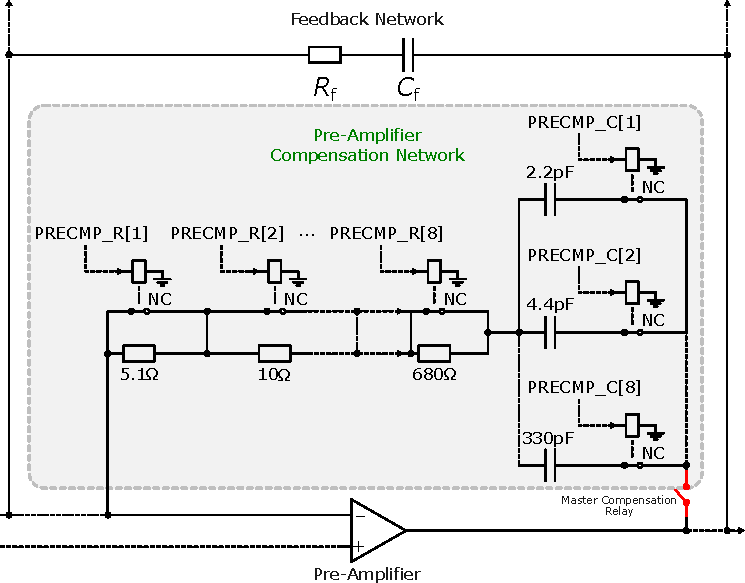
\includegraphics[width=0.9\textwidth]
    {figures/design-realization/compensation-arrangement}
    \caption[Pre-Amplifier Compensation Network]{
        Arrangement of series resistor-capacitor compensation network
        for the pre-amplifier (the power amplifier has a similar arrangement).
        A Master relay is used to enable/disable the network completely, based
        on configuration registers.
        Each component in the network has a dedicated \ac{NC} analog switch
        that is controlled by the \ac{FPGA}.
        A Wide range of R-C values can be achieved by series and parallel
        combination of the components in the network.
    }
    \label{fig:compensation-arrangement}
\end{figure}

The complete list of compensation network resistor and capacitor values
and their associated registers is given in
\hyperref[sec:compensation-network-values]{Appendix B}.
